\documentclass[a4paper]{article}

\input{style/ch_xelatex.tex}
\input{style/scala.tex}

\graphicspath{ {images/} }
\usepackage[fontset=none]{ctex}
\usepackage{graphicx}
\usepackage{color,framed}%文本框
\usepackage{listings}
\usepackage{caption}

\usepackage{hyperref}
\hypersetup{hidelinks,
	colorlinks=true,
	allcolors=black,
	pdfstartview=Fit,
	breaklinks=true}


\usepackage{amssymb}
\usepackage{enumerate}
\usepackage{xcolor}
\usepackage{bm} 
\usepackage{lastpage}%获得总页数
\usepackage{fancyhdr}
\usepackage{tabularx}  
\usepackage{geometry}
\usepackage{minted}
\usepackage{graphics}
\usepackage{subfigure}
\usepackage{float}
\usepackage{pdfpages}
\usepackage{pgfplots}
\pgfplotsset{width=10cm,compat=1.9}
\usepackage{multirow}
\usepackage{footnote}
\usepackage{booktabs}
\usepackage{listings}
\usepackage{seqsplit}
\usepackage[table]{xcolor}
\usepackage{array}
%-----------------------伪代码------------------
\usepackage{algorithm}  
\usepackage{algorithmicx}  
\usepackage{algpseudocode}  
\floatname{algorithm}{Algorithm}  
\renewcommand{\algorithmicrequire}{\textbf{Input:}}  
\renewcommand{\algorithmicensure}{\textbf{Output:}} 
\usepackage{lipsum}  
\makeatletter
\newenvironment{breakablealgorithm}
  {% \begin{breakablealgorithm}
  \begin{center}
     \refstepcounter{algorithm}% New algorithm
     \hrule height.8pt depth0pt \kern2pt% \@fs@pre for \@fs@ruled
     \renewcommand{\caption}[2][\relax]{% Make a new \caption
      {\raggedright\textbf{\ALG@name~\thealgorithm} ##2\par}%
      \ifx\relax##1\relax % #1 is \relax
         \addcontentsline{loa}{algorithm}{\protect\numberline{\thealgorithm}##2}%
      \else % #1 is not \relax
         \addcontentsline{loa}{algorithm}{\protect\numberline{\thealgorithm}##1}%
      \fi
      \kern2pt\hrule\kern2pt
     }
  }{% \end{breakablealgorithm}
     \kern2pt\hrule\relax% \@fs@post for \@fs@ruled
  \end{center}
  }
\makeatother
%------------------------代码-------------------
\RequirePackage{listings}
\RequirePackage{xcolor}
\definecolor{dkgreen}{rgb}{0,0.6,0}
\definecolor{gray}{rgb}{0.5,0.5,0.5}
\definecolor{mauve}{rgb}{0.58,0,0.82}
\lstset{
	numbers=left,  
	frame=tb,
	aboveskip=3mm,
	belowskip=3mm,
	showstringspaces=false,
	columns=flexible,
	framerule=1pt,
	rulecolor=\color{gray!35},
	backgroundcolor=\color{gray!5},
	basicstyle={\ttfamily},
	numberstyle=\tiny\color{gray},
	keywordstyle=\color{blue},
	commentstyle=\color{dkgreen},
	stringstyle=\color{mauve},
	breaklines=true,
	breakatwhitespace=true,
	tabsize=3,
}

%-------------------------页面边距--------------
\geometry{a4paper,left=2.3cm,right=2.3cm,top=2.7cm,bottom=2.7cm}
%-------------------------页眉页脚--------------
\usepackage{fancyhdr}
\pagestyle{fancy}
\lhead{\kaishu 数据安全}
\chead{密态数据库实践} 
\rhead{2312966 林晖鹏}
\lfoot{}
\cfoot{\thepage}
\rfoot{}
\renewcommand{\headrulewidth}{0.1pt}  
\renewcommand{\footrulewidth}{0pt}
\newcommand{\HRule}{\rule{\linewidth}{0.5mm}}
\newcommand{\HRulegrossa}{\rule{\linewidth}{1.2mm}}
\setlength{\textfloatsep}{10mm}
\newcolumntype{Y}{>{\centering\arraybackslash\ttfamily}X}
\newcommand{\codewrap}[1]{\texttt{\seqsplit{#1}}}

\usepackage{indentfirst}  
\setlength{\parindent}{2em}  
\linespread{1.5}  
\setCJKmainfont{Songti SC}
\setCJKsansfont{Heiti SC}
\setCJKmonofont{Songti SC}
\setCJKfamilyfont{labkai}{simkai.ttf}[Path=./]
\newcommand{\kaishu}{\CJKfamily{labkai}}

%--------------------文档内容--------------------

\begin{document}
\renewcommand{\contentsname}{目\ 录}
\renewcommand{\appendixname}{附录}
\renewcommand{\appendixpagename}{附录}
\renewcommand{\refname}{参考文献} 
\renewcommand{\figurename}{图}
\renewcommand{\tablename}{表}
\renewcommand{\today}{\number\year 年 \number\month 月 \number\day 日}

%-------------------------封面----------------

\renewcommand {\thefigure}{\thesection{}.\arabic{figure}}
\cfoot{\thepage\ of \pageref{LastPage}}

\newpage
\begin{center}
    \huge{\textbf{《数据安全》实验报告}}\\
    \vspace {0.5em}
    \Large {\textbf {密态数据库实践（FH-OPE 复现）}}
\end{center}

\begin{center}
    \textbf{姓名}：\underline{林晖鹏} \quad
    \textbf{学号}：\underline{2312966} \quad
    \textbf{专业}：\underline{计算机科学与技术}
\end{center}

\vspace{1em} 

\tableofcontents

\newpage

%--------------------------Section 1--------------------------------
\section{实验要求}
本次实验参照教材第 6.3.3 节 FH-OPE 实现展开，实验内容如下：
\begin{enumerate}
    \item 复现 FH-OPE 的基本工作流程，完成 Client、Server 编码树和 MySQL 三部分的联通；
    \item 验证系统能够完成随机化加密、密文插入和范围查询；
    \item 修改测试逻辑，对同一明文连续插入多次，观察编码树中的 recode 与 rebalance 现象。
\end{enumerate}

%--------------------------Section 2--------------------------------
\section{实验原理}
\subsection{FH-OPE 的基本思想}
FH-OPE（Frequency-Hiding Order-Preserving Encryption）的目标是在保留范围查询能力的同时，削弱重复明文的频率泄露。它不为每个明文固定分配一个唯一标签，而是把数据维护为一个动态有序序列：Client 根据明文决定插入秩位置，Server 按该秩把密文插入编码树，并分配可比较的 \texttt{encoding}。数据库中保存的是 \texttt{(encoding, ciphertext)}，查询时只依赖编码顺序，不直接接触明文。

与普通 OPE 相比，FH-OPE 的关键差异在于：同一明文不会总被插入到同一个确定位置，而是在合法区间内随机选秩插入。这样，相同明文虽然仍对应同一有序区间，但在数据库中的分布不再是完全固定的连续块，从而降低服务器直接观察频率分布的能力。

\subsection{系统结构}
本实验的实现可分为三层：
\begin{enumerate}
    \item \textbf{Client 层}：负责 AES-CBC 随机化加密、维护本地频率表、计算新记录的插入位置，并向数据库发起插入与查询请求；
    \item \textbf{Server 编码树层}：负责按照秩定位插入位置、分配 \texttt{encoding}、在必要时执行 recode 或 rebalance；
    \item \textbf{MySQL 层}：通过 UDF 调用 C++ 编码树接口，并借助存储过程把“插入 + 必要时批量更新”组织成一次数据库操作。
\end{enumerate}

三层之间的协作关系为：Client 负责决定插入秩位置，编码树负责维护全局有序编码，MySQL 负责保存密文记录并在 recode 后完成受影响记录的同步更新。

\begin{figure}[t]
    \centering
    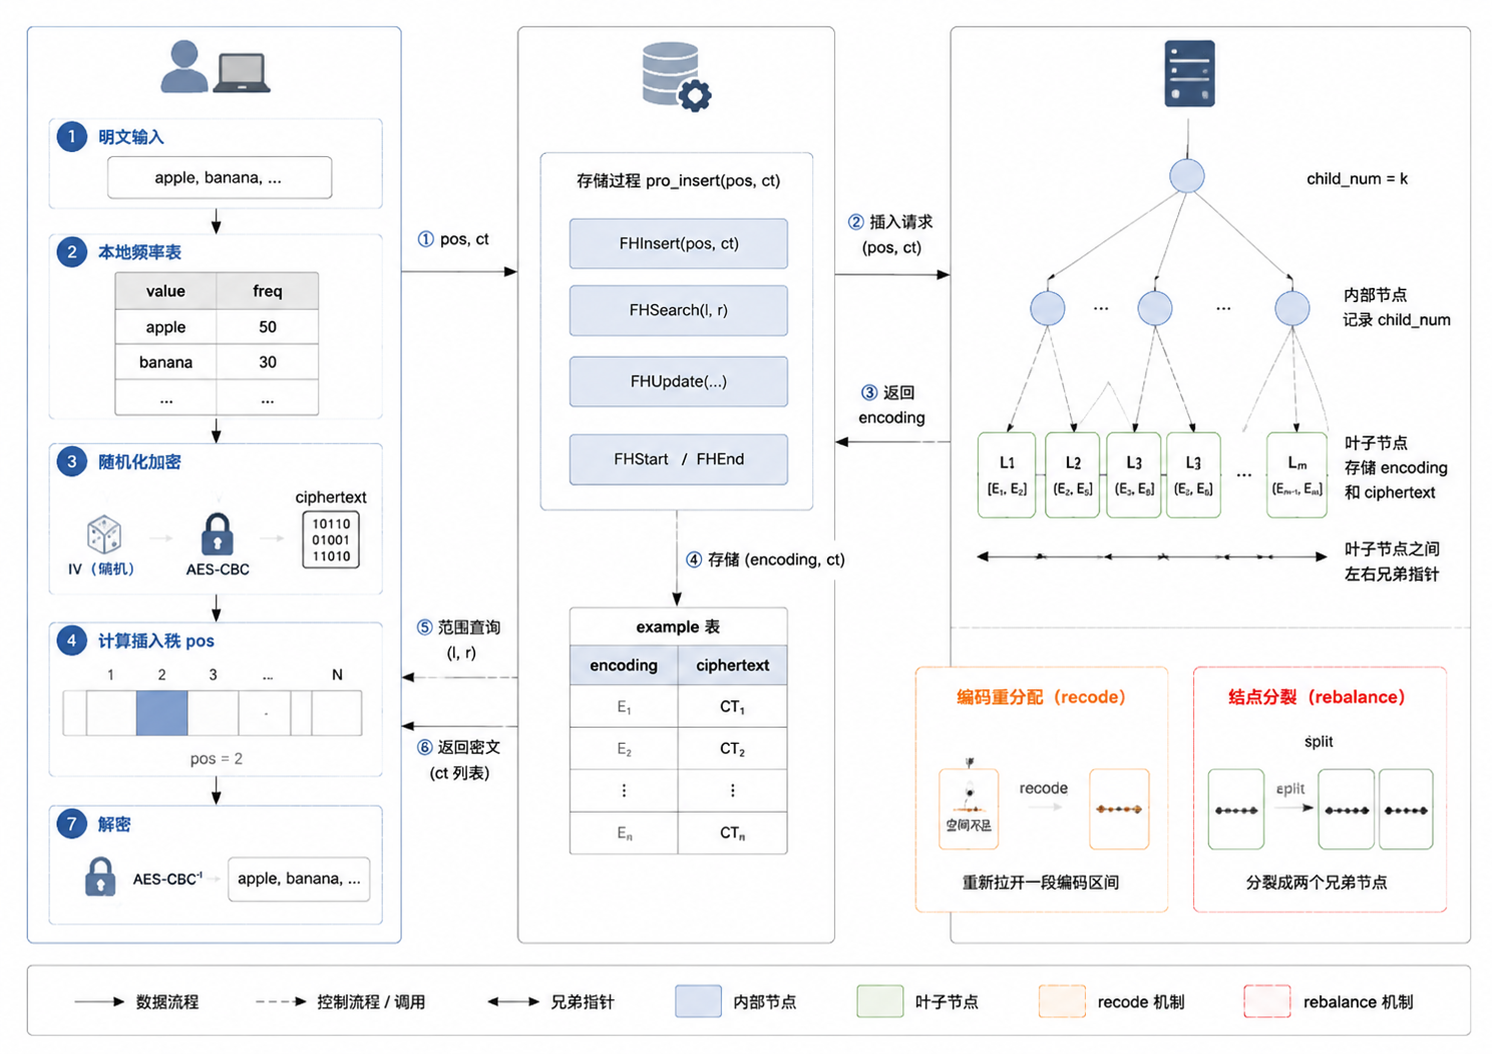
\includegraphics[width=\textwidth]{images/系统架构与加密流程图.png}
    \caption{FH-OPE 系统结构与工作流程示意图}
    \label{fig:system_workflow}
\end{figure}

图~\ref{fig:system_workflow} 展示了本实验的整体工作流程。左侧为 Client 端，负责明文输入、本地频率表维护、随机化加密和插入位置计算；中间为 MySQL 与 UDF 接口层，负责调用 \texttt{FHInsert}、\texttt{FHSearch}、\texttt{FHUpdate} 等函数，并将 \texttt{(encoding, ciphertext)} 写入数据库；右侧为编码树结构，展示了内部结点、叶子结点以及兄弟指针的组织方式。图中同时给出了 recode 与 rebalance 的示意，便于直观理解二者在 FH-OPE 中分别承担的作用。

\subsection{编码树与动态维护机制}
Server 端维护一棵多叉平衡树。内部结点记录各子树中的密文数量，用于根据秩快速下沉定位；叶子结点按顺序保存密文和编码，同时维护可分配的编码区间。这样，当 Client 给出插入秩 \texttt{pos} 时，Server 可以直接找到目标叶子并尝试插入。

在这一过程中有两个核心机制：
\begin{enumerate}
    \item \textbf{recode}：当目标位置左右编码之间已经没有足够间隙时，系统重新拉开一段区间内记录的编码，使局部重新获得可插入空间；
    \item \textbf{rebalance}：当某个叶子或内部结点达到容量阈值时，系统分裂结点并调整父结点信息，以维持树结构的平衡和检索效率。
\end{enumerate}

其中，recode 解决的是编码空间不足问题，rebalance 解决的是结点容量过满问题。二者分别对应编码维护与树结构维护两个层面。

\subsection{数据库联动机制}
为了把编码树逻辑接入数据库，本实验将 Server 端功能封装为 MySQL UDF。核心接口包括：
\begin{enumerate}
    \item \texttt{FHInsert(pos, ct)}：按秩插入密文，返回编码；若返回 0，则表示本次插入触发 recode；
    \item \texttt{FHSearch(pos)}：返回第 \texttt{pos} 个有序位置对应的编码，用于构造范围查询边界；
    \item \texttt{FHUpdate(ct)}：在 recode 后，根据密文获取其新编码；
    \item \texttt{FHStart()/FHEnd()}：返回本次 recode 影响的编码区间。
\end{enumerate}

在数据库侧，一次插入被封装为存储过程 \texttt{pro\_insert}。正常情况下，\texttt{FHInsert} 直接返回新编码，数据库把新记录写入表中；若返回 0，则说明部分旧记录的编码已经被重分配，数据库还需要根据 \texttt{FHStart()}、\texttt{FHEnd()} 和 \texttt{FHUpdate()} 对受影响区间做一次批量更新。

\begin{lstlisting}[language=SQL,caption={存储过程逻辑（节选）}]
create procedure pro_insert(IN pos int, IN ct varchar(512)) BEGIN
DECLARE i BIGINT default 0;
SET i = FHInsert(pos, ct);
insert into example values (i, ct);
if i = 0 then
update example
set encoding = FHUpdate(ciphertext)
where (encoding >= FHStart() and encoding < FHEnd()) or (encoding = 0);
end if;
END $$
\end{lstlisting}

\subsection{实验中的实现与调整}
本实验在原有代码框架基础上主要完成了以下工作：
\begin{enumerate}
    \item 梳理编码树、UDF 与 Client 的调用关系，确认插入和查询链路；
    \item 完成 UDF 编译与注册，使 MySQL 能直接调用 C++ 编码树；
    \item 在 Client 中补充或整理重复插入同一明文的测试逻辑；
    \item 加入调试日志与 CSV 导出，便于统计 recode、rebalance 及更新区间大小。
\end{enumerate}

为了在有限实验规模下更直观地观察 recode 现象，实验中将编码空间由原始的 $2^{62}$ 暂时缩小为 $2^9=512$，并加入上界截断保护，叶子容量阈值保持 $M=128$。因此，后文中关于 recode 频率和更新范围的统计结果主要用于分析机制行为，不直接对应原始参数下的系统负载情况。

%--------------------------Section 3--------------------------------
\section{实验过程}
\subsection{实验环境}
实验环境为 Ubuntu + MySQL + Python3。Server 端通过 \texttt{g++} 编译 UDF 动态库，Client 端使用 \texttt{pycryptodome} 完成 AES-CBC 加密，使用 \texttt{pymysql} 与数据库交互。完整操作流程见 \texttt{VmGuide.md}，本实验主要按以下顺序完成环境配置与系统接入：
\begin{enumerate}
    \item 安装 MySQL、编译依赖和 Python 依赖；
    \item 编译 \texttt{libfhope.so}，加载到 MySQL 插件目录；
    \item 导入 \texttt{fhope.sql}，创建 \texttt{example} 表和相关 UDF/存储过程；
    \item 运行 Client，执行基本插入、范围查询和重复插入测试。
\end{enumerate}

首先将实验目录放入虚拟机工作路径，例如 \texttt{\textasciitilde/lab4/}，随后安装 MySQL、编译依赖与 Python 依赖，命令如下：

\begin{lstlisting}[language=bash,caption={环境准备命令}]
sudo apt update
sudo apt install -y mysql-server libmysqlclient-dev g++
sudo apt install -y python3 python3-pip
pip3 install pycryptodome pymysql
\end{lstlisting}

\begin{figure}[H]
    \centering
    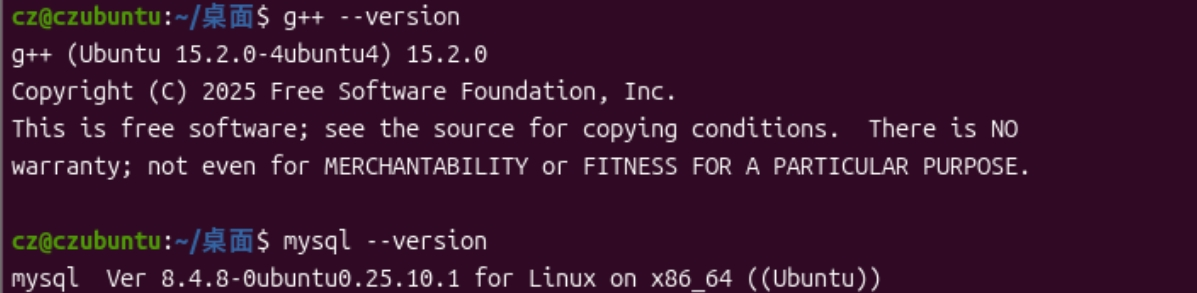
\includegraphics[width=0.9\textwidth]{images/env_done.jpg}
    \caption{实验环境配置结果}
    \label{fig:env_done}
\end{figure}

环境安装完成后，进一步创建 MySQL 用户并验证数据库连接：

\begin{lstlisting}[language=SQL,caption={创建 MySQL 用户}]
CREATE USER 'user'@'%' IDENTIFIED BY '123456';
GRANT ALL PRIVILEGES ON *.* TO 'user'@'%';
FLUSH PRIVILEGES;
\end{lstlisting}

\begin{lstlisting}[language=bash,caption={验证 MySQL 连接}]
mysql -uuser -p123456 -e "SELECT 1;"
\end{lstlisting}

\begin{figure}[H]
    \centering
    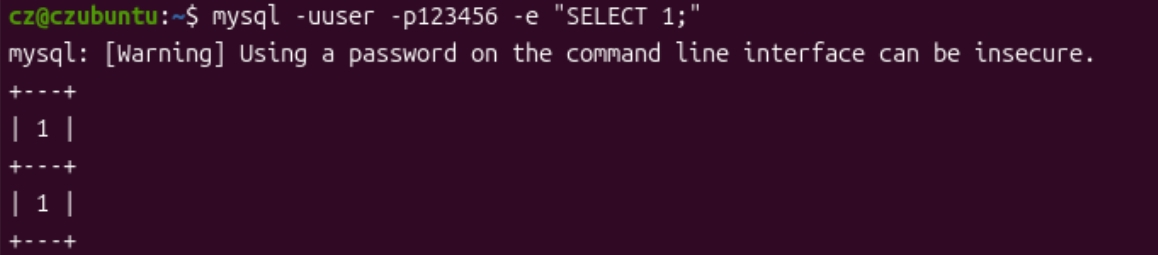
\includegraphics[width=0.9\textwidth]{images/创建MySQL用户并验证.jpg}
    \caption{MySQL 用户创建与连接验证结果}
    \label{fig:mysql_user_check}
\end{figure}

图~\ref{fig:mysql_user_check} 表明数据库用户创建成功，且客户端能够正常连接 MySQL。随后编译 UDF 动态库并接入 MySQL：

\begin{lstlisting}[language=bash,caption={编译并安装 UDF}]
cd ~/lab4
g++ -shared -fPIC UDF.cpp Node.cpp -o libfhope.so $(mysql_config --cflags) $(mysql_config --libs)
sudo cp libfhope.so $(mysql_config --plugindir)/
sudo systemctl restart mysql
\end{lstlisting}

\begin{figure}[H]
    \centering
    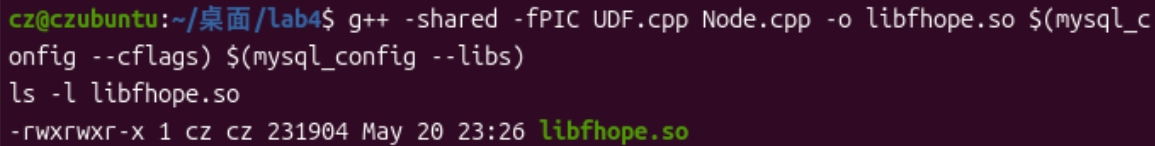
\includegraphics[width=0.9\textwidth]{images/编译完成.jpg}
    \caption{UDF 动态库编译结果}
    \label{fig:udf_build_done}
\end{figure}

图~\ref{fig:udf_build_done} 表明动态库已经成功生成。随后在数据库中导入实验 SQL 文件，创建数据表、UDF 以及存储过程接口：

\begin{lstlisting}[language=bash,caption={导入 SQL 并初始化数据库}]
mysql -uuser -p123456 << 'EOSQL'
CREATE DATABASE IF NOT EXISTS test_db;
USE test_db;
SOURCE ~/lab4/fhope.sql;
SELECT FHStart(), FHEnd();
EOSQL
\end{lstlisting}

\begin{figure}[H]
    \centering
    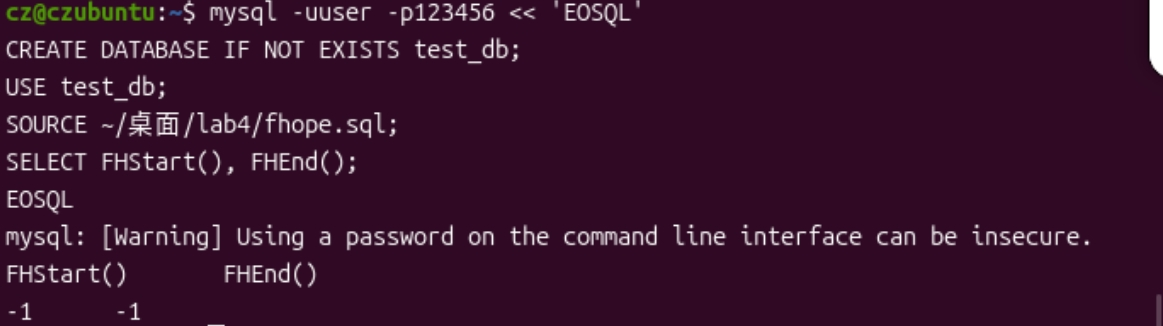
\includegraphics[width=0.9\textwidth]{images/接入验证.jpg}
    \caption{数据库初始化结果}
    \label{fig:初始化数据库成功}
\end{figure}

由图~\ref{fig:初始化数据库成功} 可见，相关函数已经能够被数据库正确识别，说明 UDF 接入成功。

\subsection{基本功能验证}
系统接入完成后，首先进行基本功能验证。Client 依次插入若干水果字符串，然后执行区间查询 \texttt{Search('b','p')}。本阶段主要验证以下内容：
\begin{enumerate}
    \item Client 能正确计算插入位置并生成随机化密文；
    \item 数据库能够通过 \texttt{pro\_insert} 和 UDF 成功维护编码顺序；
    \item 返回的查询结果经 Client 解密后与预期明文范围一致。
\end{enumerate}

首先进行单条插入测试，确认系统能够正确返回编码值：

\begin{lstlisting}[language=bash,caption={单条插入测试}]
cd ~/lab4
python3 client.py --value apple --repeat 1 --seed 1
\end{lstlisting}

随后进行多样本插入和范围查询测试：

\begin{lstlisting}[language=Python,caption={多样本插入与范围查询测试}]
import client as c
c.local_table = {}
c.key = c.get_random_bytes(16)
c.base_iv = c.get_random_bytes(16)
for fruit in ['apple', 'banana', 'cherry', 'date', 'apple', 'banana']:
    r = c.Insert(fruit)
    print(f'insert {fruit}: pos={r["pos"]} enc={r["encoding"]} recode={r["encoding"]==0}')
print()
print('=== range query [banana, cherry] ===')
c.Search('banana', 'cherry')
\end{lstlisting}

\subsection{重复插入测试}
在完成基本联通验证后，进一步对同一明文 \texttt{"apple"} 连续插入，分别测试 $N \in \{50,200,500\}$ 三组规模。每组实验开始前均重启 MySQL 并清空数据表，以保证编码树状态相互独立，从而便于对不同规模下的 recode 与 rebalance 现象进行比较。

实验中记录三类信息：
\begin{enumerate}
    \item Client 侧输出中 \texttt{enc=0} 的次数，用于统计用户可见的 recode；
    \item MySQL \texttt{error.log} 中 \texttt{FHOPE-DEBUG} 日志条目，用于统计 Server 侧 recode 与 rebalance；
    \item CSV 中每轮插入的编码、更新区间和受影响行数，用于后续分析现象演化过程。
\end{enumerate}

通过该测试，可以较清楚地观察 FH-OPE 在重复值持续插入场景下的动态行为：
\begin{enumerate}
    \item 当编码间隙不足时，观察 recode 如何扩展更新区间；
    \item 当叶子容量逼近阈值 $M=128$ 时，观察 rebalance 如何分裂树结构。
\end{enumerate}

重复插入测试使用 \texttt{--debug} 输出 C++ 侧调试日志，使用 \texttt{--csv} 保存每轮实验结果。各组实验命令如下：

\begin{lstlisting}[language=bash,caption={重复插入测试命令}]
sudo systemctl restart mysql
mysql -uuser -p123456 -e "TRUNCATE TABLE test_db.example;"
cd ~/lab4
python3 client.py --value apple --repeat 50 --seed 1 --report-every 0 --debug --csv N50.csv

sudo systemctl restart mysql
mysql -uuser -p123456 -e "TRUNCATE TABLE test_db.example;"
python3 client.py --value apple --repeat 200 --seed 1 --report-every 0 --debug --csv N200.csv

sudo systemctl restart mysql
mysql -uuser -p123456 -e "TRUNCATE TABLE test_db.example;"
python3 client.py --value apple --repeat 500 --seed 1 --report-every 1 --debug --csv N500.csv
\end{lstlisting}

其中，$N=500$ 的测试保留逐轮输出，便于从日志中直接观察 \texttt{enc=0} 的出现位置以及更新区间变化。实验完成后，再通过 MySQL 日志提取 recode 与 rebalance 事件：

\begin{lstlisting}[language=bash,caption={查看 C++ 侧调试日志}]
sudo tail -1000 /var/log/mysql/error.log | grep FHOPE-DEBUG
\end{lstlisting}

%--------------------------Section 4--------------------------------
\section{实验结果与分析}
\subsection{基本功能验证}
在基本测试中，整个调用链为：Client 计算插入位置并加密明文 $\rightarrow$ 数据库存储过程 \texttt{pro\_insert} $\rightarrow$ MySQL UDF 调用编码树插入 $\rightarrow$ \texttt{example} 表落盘 $\rightarrow$ \texttt{FHSearch} 返回编码边界 $\rightarrow$ Client 解密验证结果。实验输出表明，插入、范围过滤与解密结果彼此一致，说明 Client、Server 与 MySQL 已完成联通，且系统具备正确的范围查询能力。

\begin{figure}[htbp]
    \centering
    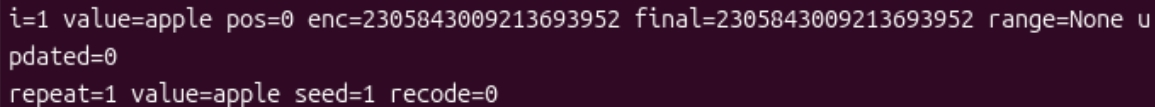
\includegraphics[width=0.9\textwidth]{images/单条插入测试.jpg}
    \caption{单条插入测试结果}
    \label{fig:single_test}
\end{figure}

% \begin{figure}[htbp]
%     \centering
%     
\includegraphics[width=0.9\textwidth]{images/basic_query.png}
%     \caption{基本插入与范围查询运行结果}
%     \label{fig:basic_run}
% \end{figure}

\begin{figure}[htbp]
    \centering
    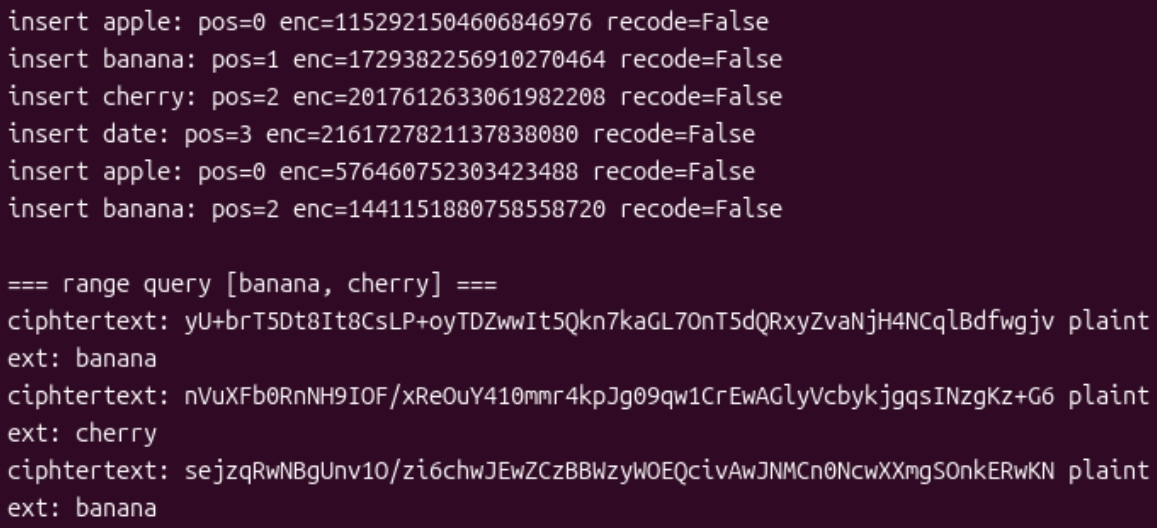
\includegraphics[width=0.9\textwidth]{images/mul_test.jpg}
    \caption{多样本插入与范围查询测试结果}
    \label{fig:mul_test}
\end{figure}

图~\ref{fig:single_test} 表明系统能够完成单条明文的加密、插入与编码返回；图~\ref{fig:mul_test} 表明数据库返回的密文结果经 Client 解密后能够恢复出正确的明文范围，说明系统已经具备正确的范围查询能力。

\subsection{重复插入测试现象分析}

实验对同一明文 \texttt{"apple"} 分别以 $N=50,200,500$ 进行连续插入，记录 recode 与 rebalance 的触发次数及关键时间点，汇总如下。


\subsubsection*{数据汇总}
\begin{table}[htbp]
    \centering
    \caption{不同插入规模下的 recode 与 rebalance 统计}
    \label{tab:recode_stats}
    \begin{tabular}{c|c|c|c|c}
        \toprule
        $N$ & rebalance次数 & recode次数 & 首次recode轮次 \\
        \midrule
        50  & 0 & 1   & round 30 \\
        200 & 1 & 12  & round 30 \\
        500 & 4 & 246 & round 30 \\
        \bottomrule
    \end{tabular}
\end{table}

从表~\ref{tab:recode_stats} 可以看出，随着插入规模的增大，recode 与 rebalance 事件均显著增加。$N=500$ 时总共约一半的插入操作触发了 recode，说明在小编码空间（$2^9=512$）下，系统承受了极高的编码更新压力。

\subsubsection*{recode 与 rebalance 的先后关系}
从统计结果可以看出，首次 recode 大约在 round 30 附近就出现，而 rebalance 的触发阈值与叶子容量 $M=128$ 相关，因此二者并不是同一类事件。前者反映的是“编码间隙已经不足”，后者反映的是“叶子结点已经装满”。这说明在本次缩小编码空间的设置下，系统首先面临的是编码空间压力，而不是树高或结点容量压力。

\subsubsection*{recode 的阶段性变化}
当 $N=500$ 时，recode 行为在时间轴上呈现出明显的阶段性特征：

\begin{enumerate}
    \item \textbf{阶段一 (round 1--30)：正常插入阶段。} 编码空间充裕，所有插入均直接分配新编码，未触发任何 recode 或 rebalance。
    \item \textbf{阶段二 (首次 recode 之后至中后期)：局部 recode 增多。} 从首次出现 \texttt{enc=0} 开始，局部编码间隙逐步被耗尽，系统开始在若干更新区间内反复执行 recode。此阶段的典型特征是：一次用户插入通常对应一次 Client 侧 recode 记录，而 Server 端可能因为更新区间扩展而执行多次内部重编码。需要强调的是，首次 recode 的出现早于首次 rebalance；二者分别由“编码间隙不足”和“叶子容量达到阈值”触发，不应混为同一事件。
    \item \textbf{阶段三 (接近末段)：大范围更新出现。} 随着编码空间进一步逼近饱和，局部 recode 能腾出的空间越来越有限，部分更新区间显著扩大。最后一次 recode 的 \texttt{updated\_rows} 达到 484，说明在该组压力测试的末段，单次插入已经可能牵动绝大部分已有记录的编码重分配。
\end{enumerate}

这种三阶段演化说明：在重复值持续进入的场景下，FH-OPE 可以通过 recode 保持顺序可插入，但代价会随着可用编码空间的减少而迅速上升。在本次实验中，recode 从零星局部修复逐步发展到接近全表范围的大规模更新。

\subsubsection*{级联 recode 现象}
一个值得注意的现象是，$N=500$ 时 Server 端 recode 次数（299 次）显著多于 Client 端记录次数（246 次），二者相差 53 次。这是因为一次用户插入虽然只触发一次 \texttt{FHInsert} 返回 0（Client 端记录一次 recode），但在编码树内部，\lstinline{Recode()} 函数可能因更新区间扩展而对多个叶子结点分别执行重编码操作，每次内部 \lstinline{Recode()} 调用都会产生一条调试日志和一次 Server 端统计。换言之，多出的 53 次源于 \textbf{级联效应}——同一插入操作在编码树内部触发了多次 \lstinline{Recode()} 调用。这一现象在编码空间局促的阶段二和阶段三尤为突出。图~\ref{fig:recode_process} 给出了重复插入过程中出现 \texttt{enc=0} 时的典型调试输出。

\begin{figure}[htbp]
    \centering
    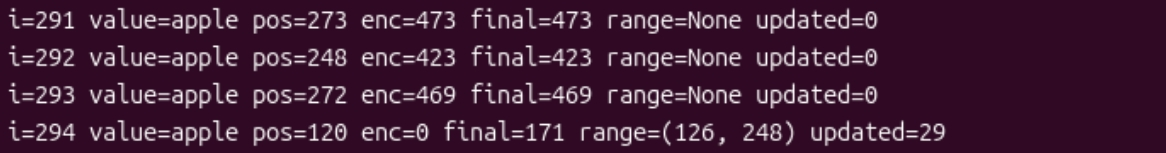
\includegraphics[width=0.9\textwidth]{images/recode_log.jpg}
    \caption{重复插入测试中的 recode 调试输出}
    \label{fig:recode_process}
\end{figure}

\subsubsection*{rebalance 触发特征}
$N=500$ 时共发生 4 次 rebalance。结合图~\ref{fig:rebalance_process} 中的 MySQL 调试日志可以看出，rebalance 的触发确实与叶子结点容量逼近阈值 $M=128$ 密切相关；但其具体发生轮次不仅取决于总插入次数，也取决于分裂后记录在各叶子之间的分布情况。因此，更稳妥的结论是：本实验观测到 rebalance 主要由局部叶子装满触发，整体次数与数据规模正相关，但不宜将其简单概括为严格的 $\lfloor N / M \rfloor$ 规律。

\begin{figure}[htbp]
    \centering
    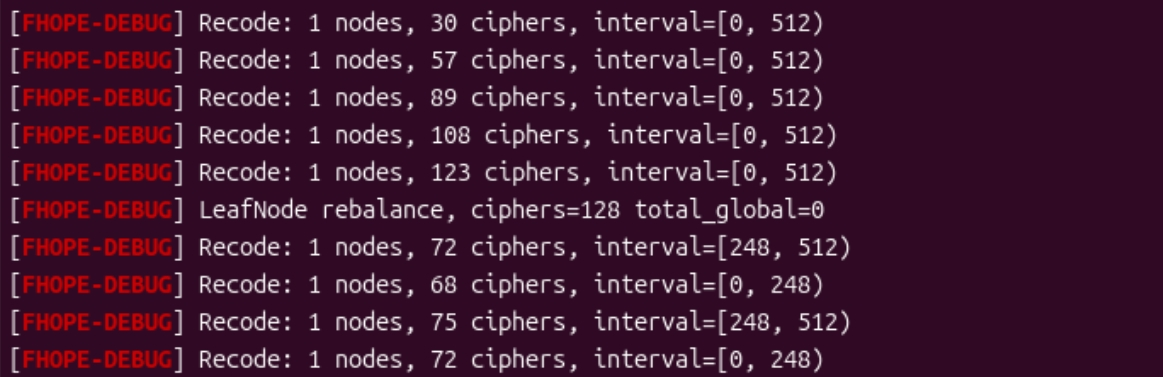
\includegraphics[width=0.9\textwidth]{images/rebalance_debug.jpg}
    \caption{MySQL 日志中的 rebalance 与 recode 事件}
    \label{fig:rebalance_process}
\end{figure}

\subsection{安全性与开销讨论}
\begin{enumerate}
    \item \textbf{频率隐藏效果}：Client 对重复明文采用随机插入位置，使得相同明文在全局有序序列中不再严格连续聚集，降低了直接频率统计的可见性。但需要注意，FH-OPE 并不等价于完全隐藏访问模式，攻击者仍可能通过长期观测与辅助信息推断部分分布特征。
    \item \textbf{系统开销}：recode 会触发数据库区间更新，其代价与更新区间长度相关；结点分裂会导致树结构调整。从定量角度看，在 $N=500$ 的这组缩小编码空间实验中，约 50\% 的插入操作触发了 Client 可见的 recode，单次 recode 最多影响 484 行记录（占全表 97\%）。这表明在编码空间接近枯竭的压力场景下，插入操作可能退化为大范围更新，系统开销不可忽略。
    \item \textbf{rebalance 规律}：本实验中共观测到 4 次 rebalance，说明随着记录数增长，树结构需要通过分裂维持检索效率。其触发机制本质上由局部叶子容量阈值控制，但具体轮次仍会受到插入位置分布和历史分裂结果的影响。
\end{enumerate}

%--------------------------Section 5--------------------------------
\section{总结}
本次实验完成了 FH-OPE 的基本复现，并成功联通了 Client、编码树 Server 逻辑与 MySQL。通过基本插入和范围查询测试，可以确认系统具备正确的密文存储与顺序查询能力；通过对同一明文的连续插入测试，可以直接观察到 recode 与 rebalance 两类动态维护机制。

实验结果表明，FH-OPE 的优势在于：它在保留范围查询能力的同时，通过随机化插入位置削弱了重复值的频率泄露；其代价在于：为了维持这一能力，系统必须在编码空间不足时执行 recode，并在结点装满时执行 rebalance。在本次缩小编码空间的压力设置下，这种代价被放大得非常明显，说明 FH-OPE 本质上是在“查询能力、频率隐藏与维护开销”之间做折中。

通过本次实验，可以较为直观地看到 FH-OPE 的工程实现方式：Client 负责秩位置计算与随机化加密，Server 负责编码树维护，数据库负责保存密文及同步更新。重复插入测试进一步说明，FH-OPE 在提供顺序查询能力的同时，需要付出额外的编码维护开销，这也是密态数据库设计中需要重点权衡的问题。

\end{document}
